\cleardoublepage

\section{理论部分}

\subsection{一些记号}
$\partial\Omega=\partial \Omega_D\cup\partial\Omega_N$: 考虑混合边界条件,如Dirichlet边界以及Neumann边界条件。 $\mathscr{T}_h$:三角化区域$\Omega$, 以尺寸 $h$为衡量标准。
$\mathscr{E}_h$:  离散化区域$\mathscr{T}_h$中所有边的集合, $\mathscr{E}_h^I$: 离散化区域$\mathscr{T}_h$中内部边的集合, $\mathscr{E}_h^D$: $\mathscr{T}_h\cap\partial\Omega_D $上边的集合, 
,$\mathscr{E}_h^N$: $\mathscr{T}_h\cap\partial\Omega_N $中边的集合。 
$\mathscr{V}_h$: 离散化区域$\mathscr{T}_h$中所有点的集合。
记$\tau$ 为$\mathscr{T}_h$中一个单元. $\Gamma=\partial \Omega$, 
$N_{\mathscr{E}}=card(\mathscr{E}_h),N_v=card(\mathscr{V}_h),N_k=card(\mathscr{T}_h)$, 
$(\cdot,\cdot)$ 和 $<\cdot, \cdot>$ 分别是 $\Omega, \Gamma$ 上的内积记号。


由于我们仅先考虑二维上的问题,因此有必要介绍一些关于向量导数的记号。

粗体字母记号,例如\textbf{u} 代表$u$为一个向量, $(u_1, u_2, \cdots u_n)$, 其中 $n=dim$. 对于 2D, $\textbf{u}=(u_1, u_2)$.\\
那么 $$\nabla \textbf{u}=\begin{pmatrix}
    {u_1}_x & {u_2}_x\\
    {u_1}_y & {u_2}_y
\end{pmatrix}, \nabla \cdot (\nabla \textbf{u})=\Delta \textbf{u}=\begin{pmatrix}
    {u_1}_{xx}+{u_1}_{yy}\\
    {u_2}_{xx}+{u_2}_{yy}\\
\end{pmatrix}$$

为了计算弱形式的方便,我们引入double product:
$$\nabla \textbf{u}:\nabla \textbf{v}=\sum_{j}\sum_{i}\frac{\partial u_i}{\partial x_j}\frac{\partial v_i}{\partial x_j}$$
和索伯列夫空间
$$\begin{aligned}
    H^1(\Omega)&=\{u\in L^2(\Omega):\partial^\alpha u\in L^2(\Omega),|\alpha|\leq 1\}\\
    H^1_0(\Omega)&=\{u\in H^1(\Omega): u|_{\partial \Omega}=0\}\\
    L^2_0(\Omega)&=\{u\in L^2(\Omega): \int_\Omega u=0\}
\end{aligned}$$

对于向量 $\textbf{u}\in [H^1_0]^n$, 
有范数 $$\left\|\textbf{u}\right\|_{H^1_0}=\left(\left\|\textbf{u}\right\|^2_{L^2(\Omega)}+\left\|\nabla \cdot \textbf{u}\right\|^2_{L^2(\Omega)}\right)^{\frac{1}{2}}$$

由于我们想要考虑NS方程上问题,首先考虑混合有限元方法。

\section{混合有限元方法(Mixed Finite Element Method)}
我们在变量耦合的地方应用MFEM。斯托克斯方程是NS方程雷诺数趋向于0的特殊情况,因此我们以斯托克斯方程作为例子。
$$\left\{
\begin{aligned}
    &-\Delta \textbf{u}+\nabla p = \textbf{f} \qquad &in\ \Omega\\
    &u=0\qquad &on \ \Gamma_D\\
    &\nabla \cdot \textbf{u} = 0\qquad &\Gamma_N\\
\end{aligned}
\right.$$
其中 $\textbf{u}=(u_1,u_2)$ 为速度场中向量, p 为压力场为标量, $\textbf{f}=(f_1, f_2)$. 困难在与如何解耦u和p这两个变量。
As we can see, if some $(\textbf{u}, p)$ solve the equations above then $(\textbf{u}, p)$ does as well. 
为了解的唯一性,我们需要施加额外条件 $\int_\Omega p=0$

因此我们可以得到斯托克斯方程的弱形式: 寻找$\textbf{u}\in V=[H^1_0]^2$ 并且 $p\in W=L^2_0$ s.t.

$$\left\{
    \begin{aligned}
        &a(\textbf{u},\textbf{v})-b(\textbf{v}, p)=(\textbf{f}, \textbf{v}) \qquad &\forall \textbf{v}\in V\\
        &b(\textbf{u}, q)=0 \qquad &\forall q\in W
    \end{aligned}
\right.$$
其中 $$\begin{aligned}
    &a(\textbf{u},\textbf{v})=(\nabla \textbf{u},\nabla \textbf{v})=\int_\Omega \nabla \textbf{u}:\nabla \textbf{v}d\Omega\\
    &b(\textbf{v}, q)=(\nabla\cdot \textbf{v}, q)=\int_\Omega \nabla\cdot \textbf{v}\cdot q
\end{aligned}$$

\subsection{优化}
我们可以把上述问题转化为一个优化问题
$$\begin{aligned}
    \textbf{u}&=arg \min_{\textbf{v}\in V, \nabla \cdot \textbf{v}=0}\left\{\frac{1}{2}\left\|\nabla \textbf{v}\right\|^2_{L^2(\Omega)}-(\textbf{f}, \textbf{v})\right\}\\
    &=arg \min_{\textbf{v}\in V} \max_{q\in W}\left\{\frac{1}{2}\left\|\nabla \textbf{v}\right\|^2_{L^2(\Omega)}-(\textbf{f}, \textbf{v}) -(\nabla \cdot \textbf{v}, q)\right\}
\end{aligned}$$

(Here i think we can apply the adverserial network to this problem. WAN is a reference.)
\subsection{离散化}

我们引入 $V_h\subset V, W_h\subset W$ 并且想要寻找$V_h$基函数 $\{\phi_1,\phi_2\cdots \phi_n\}$,  $W_h$中基函数$\{\psi_1, \psi_2\cdots \psi_m\}$. 
因此我们需要寻找 $(\textbf{u}_h, p_h)\in V_h\times W_h$, 更具体的是, $\textbf{u}_h=\sum_i\textbf{U}(\textbf{x}_i)\phi_i$ 和 $p=\sum_iP(\textbf{x}_i)\psi_i$ s.t. 

$$\left\{
\begin{aligned}
    &a(\textbf{u}^h, \textbf{v}^h)-b(\textbf{v}^h,p^h)=(\textbf{f}, \textbf{v}) \qquad &\forall \textbf{v}^h\in V_h\\
    &b(\textbf{u}^h, q^h)=0\qquad &\forall q\in W^h
\end{aligned}
\right.$$

因此我们得到
$$\left\{
    \begin{aligned}
        &AU-BP=F\\
        &B^TU=0
    \end{aligned}
\right.\quad\text{i.e.}\quad 
\begin{pmatrix}
    A & -B\\
    B^T & 0
\end{pmatrix}\begin{pmatrix}
    U\\P
\end{pmatrix}=\begin{pmatrix}
    F\\0
\end{pmatrix}$$
其中 $A=(a_{ij}),a_{ij}=a(\phi_i, \phi_j)=(\nabla \phi_i, \nabla \phi_j);B=(b_{ij}),b_{ij}=b(\phi_j, \psi_i)=(\psi_i, \nabla\cdot\phi_j);F=(F_i),F_i=(\textbf{f},\phi_i)$

这是解决斯托克斯方程的混合有限元方法,它一个和时间无关的静态方程,然而对于许多PDE问题而言往往是瞬态方程。所以如何处理时间变量是一个重要的问题。
时间项处理的好坏直接影响着结果的优劣,一些经典问题如误差累积,以及并行计算的困难等等。

\section{间断有限元方法(Discontinuous Galerkin Method)}\label{Interior Penalty Discontinuous Galerkin Method}
间断有限元方法是最先被设计用于解决双曲守恒定律的经典数值算法,在近些年里逐渐变得流行,其主要特点在于允许解有间断性,这在解决拥有间断,突变解的问题上有着很大的优势。
我们选择间断有限元方法主要是由于它拥有普通有限元方法不具备的灵活性,例如
\begin{itemize}
    \item 允许利用任意已知点进行三角划分
    \item 在每个单元上可以自由的选择用于拟合的多项式的次数
    \item 局部精确收敛
    \item 可以实现很高效率的并行计算 
\end{itemize}

我们利用内罚间断有限元方法(Interior Penalty Discontinuous Galerkin Method)以解决Possion方程为例,我们首先有如下定义:跳量和平均量
$$\left\{
    \begin{aligned}
        &[u]_{kl}=(u|_{\tau_k}-u|_{\tau_l})\\
        &{u}= \frac{1}{2}(u|_{\tau_k}+u|_{\tau_l})
    \end{aligned}
\right.$$

\begin{definition}
    (\textbf{Broken Sobolev space})
    对于  $s \geq 0$  broken Sobolev space为
    $$H^{p}\left(\mathscr{T}_h\right):=\left\{v \in L_{2}(\Omega): v|_{\tau} \in H^{p}\left(\tau\right) \text { for all } \tau \in \mathscr{T}_h\right\}$$
    有分片p阶多项式组成的离散函数空间为
    $$S^p_h(\mathscr{T}_h):=\{v_h\in L_2(\Omega):v_h|_{\tau}\in\mathbb{P}_p(\tau),\forall \tau \in \mathscr{T}_h\}$$
\end{definition}

限制在 $\tau \in \mathscr{T}_h$ 属于索伯列夫空间 并且在$\tau$的内部边界上不连续。

\subsection{Possion方程}
考虑有混合边界的Possion方程,有如下形式:
$$\left\{\begin{aligned}
    &-\nabla\cdot(a(\nabla u))=f\qquad x \in \Omega\\
    &u=g_D \qquad x\in\Gamma_D\\
    &u=g_N \qquad x\in\Gamma_N
\end{aligned}\right.$$

在这里我们假设 $g_D=0$. 我们将其画为弱解形式: 对于 $\forall v\in V:=\{v|_\tau\in H^2(\tau),\forall \tau\in \mathscr{T}_h\}$
$$\begin{aligned}
(f, v) & =-\int_{\Omega} \nabla \cdot(a \nabla u) v=-\sum_{\tau \in \mathscr{T}_{h}} \int_{\tau} \nabla \cdot(a \nabla u) v \\
& =\sum_{\tau \in \mathscr{T}_{h}} \int_{\tau} a \nabla u \cdot \nabla v-\sum_{\tau \in \mathscr{T}_{h}} \int_{\partial \tau} a \textbf{n}_{\tau}\cdot \nabla u  v .
\end{aligned}$$

\begin{theorem}(\textbf{Sobolev Embedding Theroem})
    若 $u\in W^{k,p}(\Omega)$, 其中 $p>1$, 当 $m:=k-\frac{n}{p}>0$, 那么 $u\in C^{m}(\Omega)$
\end{theorem}

那么如果 $u\in H^2(\Omega)$, 所以 $u\in C^m(\Omega)$,即 $[u]=[\nabla u]=0$

因此我们有
$$\begin{aligned}
\sum_{\tau \in \mathscr{T}_{h}} \int_{\partial \tau} a & \nabla u \cdot \textbf{n}_{\tau} v=\sum_{e \in \mathcal{E}_{h}^{I}} \int_{e}[a \textbf{n}\cdot \nabla u  v] +\sum_{e \in \mathcal{E}_{h}^{D}} \int_{e} a\textbf{n}\cdot \nabla u  v + \sum_{e \in \mathcal{E}_{h}^{N}} \int_{e} a \textbf{n}\cdot \nabla u  v \\
& =\sum_{e \in \mathcal{E}_{h}^{I}} \int_{e}([a \nabla u \cdot \textbf{n}]\{v\}+\{a \nabla u \cdot \textbf{n}\}[v])+\sum_{e \in \mathcal{E}_{h}^{D}} \int_{e} a \nabla u \cdot \textbf{n} v +\int_{\Omega_N}g_Nv\\
& =\langle\{a \nabla u \cdot \textbf{n}\},[v]\rangle_{\mathcal{E}_{h}^{I D}}+\int_{\Omega_N}g_Nv
\end{aligned}$$

所以
$$(a \nabla u, \nabla v)_{\mathscr{T}_{h}}-\langle\{a \nabla u \cdot \textbf{n}\},[v]\rangle_{\mathcal{E}_{h}^{I D}}=(f, v)_{\mathscr{T}_h}+\int_{\Omega_N}g_Nv, \quad \forall v \in V .$$

为了对称性考虑,并且添加惩罚项,我们定义双线性型:
$$\left\{\begin{aligned}
    &A_{h}(u, v):=  (a \nabla u, \nabla v)_{\mathscr{T}_{h}}-\left(\langle\{a\textbf{n}\cdot \nabla u \},[v]\rangle_{\mathcal{E}_{h}^{I D}}-\epsilon\langle\{a \textbf{n}\cdot\nabla v \}, [u]\rangle_{\mathcal{E}_{h}^{I D}}\right)+J_{0}(u, v)+J_{1}(u, v)\\
    &F_h(v)=(f, v)_{\mathscr{T}_h}+\int_{\Omega_N}g_Nv+\epsilon\langle\{a \textbf{n}\cdot\nabla v \}, [u]\rangle_{\mathcal{E}_{h}^{D}}, \quad \forall v \in V
\end{aligned}\right.$$
其中 $$J_{0}(u, v):= \sum_{e \in \mathcal{E}_{h}^{I D}} \frac{\sigma_{0}}{h_{e}} \int_{e}[u][v],\qquad
J_{1}(u, v):= \sum_{e \in \mathcal{E}_{h}^{I}} \sigma_{1} h_{e} \int_{e}[a \nabla u \cdot n][a \nabla v \cdot n]$$

注意到对于精确解 $u$ 而言,我们自然的有 
$$\left\{\begin{aligned}
    &\epsilon\langle\{a \textbf{n}\cdot\nabla v \}, [u]\rangle_{\mathcal{E}_{h}^{I D}}=\epsilon\langle a \textbf{n}\cdot\nabla v, u\rangle_{\mathcal{E}_{h}^{D}}\\
    &J_{0}(u, v)= \sum_{e \in \mathcal{E}_{h}^{D}} \frac{\sigma_{0}}{h_{e}} \int_{e}g_Dv
\end{aligned}\right.$$


因此对于这里拥有齐次边界条件的精确解 $u$来说, 我们显然有
$$\langle\{a \nabla v \cdot n\},[u]\rangle_{\mathcal{E}_{h}^{I D}}=J_{0}(u, v)=J_{1}(u, v)=0, \quad \forall v \in V$$

因此我们需要找到 $ u_{h} \in S_h^p(\mathscr{T}_h)$ s.t.

$$A_{h}\left(u_{h}, v_{h}\right)=F_h(v_h) \quad \forall v_{h} \in S_h^p(\mathscr{T}_h) .$$

之后我们只要项平常的有限元方法一样寻找基函数即可。上边所离散的问题等价于一个线性方程组的问题,我们可以通过合适的直接的或者间接的方法解决。
例如我们设$u_h=\sum_{i=1}^{N_h}u_i\phi_i$, 那么 
$$\sum_{i=1}^{N_h}A_h(\phi_j,\phi_i)u_i=F_h(\phi_j),j=1\cdots N_h$$
这可以被写作为矩阵形式 $AU=F$


\section{瞬态问题(Time-dependent problems)}
事实上我们有三种方法解决这些问题。
\begin{itemize}
    \item 对于时间项,使用差分方法,如单步法,线性多步法,来进行时间步长迭代
    \item 空间维度用有限元方法进行时间离散,最后将PDE系统化为为ODE系统
    \item 利用时空有限元方法(STFEM)同时离散空间和时间维度;
\end{itemize}

因此我们基于NS方程分别讨论了这三种方法。在这里,我们仅考虑其次Dirichlet边界条件,$\Omega$ 为空间区域,$I=(0,T)$ 为时间域:
$$\left\{
    \begin{aligned}
        &\textbf{u}_t+(\textbf{u}\cdot \nabla)\textbf{u}+\frac{1}{\rho}\nabla p-\gamma \Delta \textbf{u}=\textbf{f}\quad \text{in} \ \Omega\times I\\
        &\nabla \cdot \textbf{u}=0\\
        &\textbf{u}|_{\partial \Omega}=0
    \end{aligned}
\right.$$

\subsection{时间差分}
首先我们尝试时间差分离散化。我们有高效的数值方法来处理时间项,如龙格库塔方法。我们以向前欧拉为例子,我们有
\begin{equation}
    \begin{aligned}
    &\frac{\textbf{u}_{n+1}-\textbf{u}_n}{\Delta t}=\gamma \Delta \textbf{u}_n-(\textbf{u}_n\cdot \nabla) \textbf{u}_n-\frac{1}{\rho}\nabla p_n+\textbf{f}\stackrel{\text{denote}}{=}\textbf{F}(\textbf{u}_n,p_n)\\
    \Rightarrow&\textbf{u}_{n+1}=\textbf{u}_n+\Delta t \textbf{F}(\textbf{u}_n,p_n)
    \end{aligned}  
    \label{1}
\end{equation}

其中 $\textbf{u}_n$ 代表在第n步的解 $\textbf{u}$ 。同时我们其他时间离散方案如 leapfrog method, RK method etc. 
然而 $\textbf{u}_{n+1}$ 可能不满足 $\nabla \cdot \textbf{u}=0$ 并且没有办法处理压力项 $p_n$. 因此我们介绍 splitting operator method.

通常我们同时有 
\begin{equation}
    \frac{\textbf{u}_{n+1}-\textbf{u}_n}{\Delta t}=\gamma \Delta \textbf{u}_n-(\textbf{u}_n\cdot \nabla) \textbf{u}_n-\frac{1}{\rho}\nabla p_{n+1}+\textbf{f}=\textbf{F}(\textbf{u}_n,p_{n+1})\\
\end{equation}
其中 $\nabla \cdot \textbf{u}_{n+1}=0$. 并且我们记 eq\ref*{1}中$\textbf{u}_{n+1}$  为 $\textbf{u}^*$. 

那么我们需要寻找一个修正 $\delta \textbf{u}$ s.t. $\textbf{u}_{n+1}=\textbf{u}^*+\delta \textbf{u}$, 所以 $\nabla \cdot \textbf{u}_{n+1}=0$.

自然的我们有
 $$\delta \textbf{u}=-\frac{\Delta t}{\rho}\nabla(p_{n+1}-\beta p_n)\stackrel{denote}{=}-\frac{\Delta t}{\rho}\nabla \Phi$$
i.e. $\Phi=p_{n+1}-p_n$. 因此 $\nabla\cdot \textbf{u}_{n+1}=\nabla \cdot(\textbf{u}*+\delta \textbf{u})=\nabla \cdot (\textbf{u}^*-\frac{\rho}{\Delta t}\nabla\Phi)=0$, 
也即
\begin{equation}
    \Delta \Phi = \frac{\rho}{\Delta t}\nabla \cdot \textbf{u}
    \label{Possion}
\end{equation} 

然后我们可以更新 $\textbf{u}_{n+1},p_{n+1}$, 通过 
\begin{equation}\left\{
    \begin{aligned}
        &\textbf{u}_{n+1}=\textbf{u}^*-\frac{\Delta t}{\rho}\nabla \Phi\\
        &p_{n+1}=\Phi + \beta p_n
    \end{aligned}\right.
\end{equation}

这是一种将复杂问题转化为简单的小问题的方法。总结一下步骤如下:
\begin{itemize}
    \item Compute $\textbf{u}^*$
    \item Solve Possion Equation \ref*{Possion}
    \item Update $\textbf{u}_{n+1}$\&$p_{n+1}$
\end{itemize}

Then we wanna get the weak form, introduce the test function $\textbf{v}^{(u)}\in V^{(u)}$\& $\textbf{v}^(\phi)\in V^{(\phi)}$. By integration by parts:
$$\begin{aligned}
    &\int_\Omega\Delta \textbf{u}\textbf{v}=-\int_\Omega\nabla\textbf{u}:\nabla\textbf{v}+\int_{\partial\Omega}\frac{\partial \textbf{u}}{\partial \textbf{n}}\cdot \textbf{v}ds\\
    &\int_\Omega \nabla p\cdot \textbf{v}=-\int_\Omega p\cdot \nabla \cdot \textbf{v}+\int_{\partial \Omega}p\cdot\textbf{n}\textbf{v}ds
\end{aligned}$$where $\frac{\partial \textbf{u}}{\partial \textbf{n}}=\textbf{n}\cdot \nabla \textbf{u}$ we have the weak form:

\begin{equation}
    \begin{aligned}
        &\int_\Omega\left[\textbf{u}^*\textbf{v}^{(u)}+\Delta t(\textbf{u}_n\cdot \nabla)\textbf{u}_n\cdot \textbf{v}_n\right]-\int_\Omega\beta \frac{\Delta t}{\rho}p^n\nabla\cdot \textbf{v}^{(u)}
        +\int_\Omega \Delta t\gamma \nabla\textbf{u}_n:\nabla \textbf{v}_n\\
        &=\int_\Omega\Delta t \gamma \textbf{f}\cdot \textbf{v} + \int_\Omega\left(\Delta t\gamma\frac{\partial \textbf{u}}{\partial \textbf{n}}\textbf{v}^{(u)}-\beta\frac{\Delta t}{\rho}p\cdot\textbf{n}\textbf{v}\right)ds\\
        &\int_{\Omega} \nabla \Phi\cdot \nabla \textbf{v}^{\phi}=-\frac{\rho}{\Delta t}\int_\Omega \nabla \cdot \textbf{u}^*\cdot \textbf{v}^{(\phi)}+\int_{\partial\Omega}\frac{\partial \Phi}{\partial \textbf{n}}\textbf{v}^{(\phi)}ds
    \end{aligned}
\end{equation}

This kind of methods suffer from error accumulation and it requires hard condition for stability. We want more continuity and less discretization.

\subsection{Convert to ODE}
We can get weak form of NS Equ directly.
\begin{equation*}\left\{
    \begin{aligned}
        &\int_\Omega \textbf{u}_t \textbf{v} + \int_\Omega \gamma \nabla \textbf{u}:\nabla\textbf{v} + \frac{1}{\rho}\int_\Omega p\nabla \cdot\textbf{v}+\int_\Omega(\textbf{u}\cdot \nabla) \textbf{u}\cdot\textbf{v}
        =\int_\Omega \textbf{f}\cdot\textbf{v}+ \int_\Omega\left(\gamma\frac{\partial \textbf{u}}{\partial \textbf{n}}\textbf{v}^{(u)}-\frac{1}{\rho}p\cdot\textbf{n}\textbf{v}\right)ds\qquad &\textbf{v}\in V\\
        &\int_\Omega \nabla\cdot \textbf{u} q=0 &q\in W
    \end{aligned}\right.
\end{equation*}

Reduced to 

\begin{equation*}\left\{
    \begin{aligned}
        &(\textbf{u}_t, \textbf{v})+\gamma a(\textbf{u}, \textbf{v})-\frac{1}{\rho}b(\textbf{v}, p)+((\textbf{u}\cdot \nabla)\textbf{u}, \textbf{v})=(\textbf{f}, \textbf{v})\\
        &b(\textbf{u}, q)=0
    \end{aligned}\right.
\end{equation*}

Set $V_h\subset V, W_h\subset W$ and the basis $\{\phi_1, \phi_2,\cdots \phi_{N_v}\}$ for $V_h$, then assume $$u^h=\sum_{i=1}^{N_v}U(t,\textbf{x}_i)\phi_i(\textbf{x})$$ and apply this to 
\begin{equation*}\left\{
    \begin{aligned}
        &(\textbf{u}^h_t, \textbf{v}^h)+\gamma a(\textbf{u}^h, \textbf{v}^h)-\frac{1}{\rho}b(\textbf{v}^h, p^h)+((\textbf{u}^h\cdot \nabla)\textbf{u}^h, \textbf{v}^h)=(\textbf{f}, \textbf{v}^h)\\
        &b(\textbf{u}^h, q^h)=0
    \end{aligned}\right.
\end{equation*}
Then reduced to a ODE system:

($...$The nonlinear term is too hard to handle, I was wondering if i should change the demo model(NS)...)

\section{Space-time FEM}
Let me introduce the space-time finite element method.
I find this method quite interesting. One big advantage of space-time methods is that they can treat moving domains in a natural way. Another advantage is that its a powerful method to 
handle problems with local singularities. In this work, we introduce the space-time methods based on Discontinuous Galerkin FEM.

To be simple, the task is to find a time-dependent basis for the space-time domain. Now NS Equ is too difficult for me to solve, so lets consider the heat equation first.
\subsection{For Heat Equation}
The heat equation with mixed boundary condition is:

$$\left\{\begin{aligned}
&c  u_t(\textbf{x}, t)-\nabla_x \cdot\left[A(\textbf{x}, t) \nabla_x u(x, t)\right]  =f(\textbf{x}, t) & \text { for }(\textbf{x}, t) \in Q:=\Omega \times(0, T), \\
&u(\textbf{x}, t) =g_D  & \text { for }(\textbf{x}, t) \in \Sigma_D:=\Gamma_D \times(0, T), \\
&\textbf{n}_x\cdot \nabla_xu=g_N & \text{ for } (\textbf{x}, t) \in \Sigma_N:=\Gamma_N \times(0, T)\\
&u(\textbf{x}, 0) =u_{0}(\textbf{x})  & \text { for } \textbf{x} \in \Omega,
\end{aligned}\right.$$

where the coefficient matrix  $A(\textbf{x}, t)=[A(\textbf{x}, t)]^{\top} \in \mathbb{R}^{n \times n}$  is positive definite uniform in  $(\textbf{x}, t) \in Q $; 
And $c>0$ is the heat capacity constant, $f \in L_{2}\left(0, T ; H^{-1}(\Omega)\right)$  is a given source term.
and we assume  $u_{0} \in H_{0}^{1}(\Omega)$.

\subsubsection*{Discretization}
Q(1D) is the space-time domain like:

\begin{center}
    \begin{tikzpicture}
        \draw[->, thick] (-1,0) -- (5,0) node[right] {$x$};  
        \draw[->, thick] (0,-1) -- (0,5) node[above] {$t$};
        \draw (0,0)--(4,0)--(4,4)--(0,4)--(0,0);
        \node at (2,4.5) {$\Sigma_T$};
        \node at (4.5,2) {$\Sigma_N$};
        \node at (-0.5,2) {$\Sigma_D$};
        \node at (2,-0.5) {$\Sigma_0$};
        \node at (4,-0.5) {$X$};
        \node at (-0.5,4) {$T$};
        \node at (2,2) {$Q$};
    \end{tikzpicture}
\end{center}

%   \cap H^{1}(0, T, H^{-1}(\Omega))
Here we only consider homogeneous pure Dirichlet boundary condition. 

This discretization scheme is based on a discontinuous Galerkin approach in space and time. 
This approach allows the use of arbitrary elements in space and time which has advantages when we have to deal with moving domains
For other discontinuous Galerkin discretization schemes in space and time, where the discretization is based on so called space-time slabs.
In this work, we will allow unstructered decompositions for the space-time domain.

We declear the discretization of Q as $Q_h$, and the basic element of $Q_h$ noted as $\tau_l$, i.e. $Q_h=\bigcup_l \tau_l $, which are triangles (n = 1),
tetrahedra (n = 2), or pentatops (n = 3), like:

\begin{figure}[H]  
    \centering  
    \includegraphics[width=0.5\textwidth]{./pics/final/p2.png}  
    \caption{Reference(structured) element and unstructured mesh}  
    % \label{fig:my_label}  
\end{figure}  

\subsubsection*{Variational Formulation}

Fist we have weak form as:

\begin{equation}
    \int_Qu_tv-\int_Q\Delta uv = \int_Q fv
\end{equation}

\begin{definition}[Interior facet]
    For two neighboring elements $\tau_k,\tau_l\in Q_h$, the interior facet $\Gamma_{kl}$ is given by
    $$e_{kl}:=\overline{\tau_k}\cap\overline{\tau_l}$$
    And the set of interior facet denoted by $\mathscr{E}_h^I$
\end{definition}

\begin{center}
    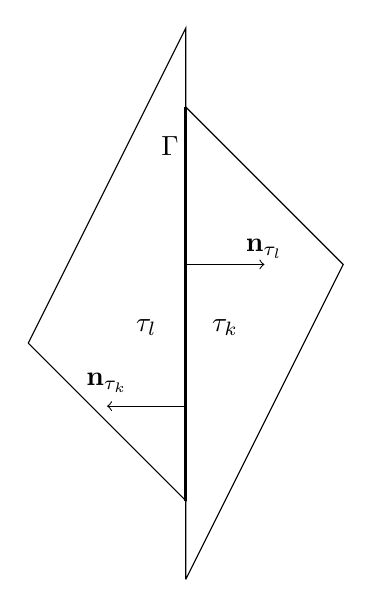
\begin{tikzpicture}
        \draw (0,2)--(2,0)--(2,6)--(0,2);
        \draw (2,-1)--(2,5)--(4,3)--(2,-1);
        \draw[line width=1pt] (2,0) -- (2,5);
        \draw[->] (2,3)--(3,3); 
        \draw[->] (2,1.2)--(1,1.2); 
        \node at (3,3.2) {$\textbf{n}_{\tau_l}$};
        \node at (1,1.5) {$\textbf{n}_{\tau_k}$};
        \node at (1.8,4.5) {$\Gamma$};
        \node at (1.5,2.2) {$\tau_l$};
        \node at (2.5,2.2) {$\tau_k$};
    \end{tikzpicture}
\end{center}

We have some definition similar to those in possion equation, but still have some differences. 

\begin{definition}[Jump and average]\label{def}
    1.The jump across the interior facet $e_{kl}$ is:
    $$[v]_{e_{k l}}:=v|_{\tau_{k}} \boldsymbol{n}_{k}+v|_{\tau_{l}} \boldsymbol{n}_{l} $$
    2.The jump in space direction:
    $$[v]_{e_{k l}, \boldsymbol{x}}:=\boldsymbol{v}|_{\tau_{k}} n_{k, \boldsymbol{x}}+\boldsymbol{v}|_{\tau_{l}} n_{l, \boldsymbol{x}} ,$$
    3.The jump in time direction:
    $$[v]_{e_{k l}, t}:=v|_{\tau_{k}} n_{k, t}+v|_{\tau_{l}} n_{l, t}  .$$
    4.The average of a function  v  on the interior facet  $e_{kl}$  is
    $$\langle v\rangle_{e_{kl}}:=\frac{1}{2}\left(v|_{\tau_{k}}+v|_{\tau_{l}}\right) ,$$
    5.The upwind in time direction:
    $$\{v\}_{e_{k l}}^{\text {up }}:=\left\{\begin{array}{ll}
        v|_{ \tau_{k}} & \text { for } n_{k, t}>0 \\
        0 & \text { for } n_{k, t}=0 \\
        v|_{ \tau_{l}} & \text { for } n_{k, t}<0
        \end{array}  .\right.$$
    6.The downwind in time direction:
    $$\{v\}_{e_{k l}}^{\text {down }}:=\left\{\begin{array}{ll}
        v|_{ \tau_{l}} & \text { for } n_{k, t}>0 \\
        0 & \text { for } n_{k, t}=0 \\
        v|_{ \tau_{k}} & \text { for } n_{k, t}<0
        \end{array}  .\right.$$
\end{definition}

Here $\textbf{n}_k$ is the unit normal vector of $\tau_k$, $n_x=\textbf{n}_k\cdot \hat{x}, n_t=\textbf{n}_k\cdot \hat{t}$. And we notice that for $e_{kl}\in \mathscr{E}_h^D,[v]=\{v\}=v$, and for $e\in \mathscr{E}_h^I,[vw]=[v]\{w\}+\{v\}[w]$

We qpproximate the laplacian $\Delta u$ by interior penalty Galerkin Method just like Possion Equation:

\begin{equation}\label{auv}
    \begin{aligned}
        a\left(u_{h}, v_{h}\right):=  &\sum_{l=1}^{N} \int_{\tau_{l}} \nabla_{x} u_{h} \cdot \nabla_{\boldsymbol{x}} v_{h} 
         -\sum_{e_{k l} \in \mathscr{E}_h^{ID}} \int_{e_{k l}}\left\langle\nabla_{\boldsymbol{x}} u_{h}\right\rangle_{e_{k l}} \cdot\left[v_{h}\right]_{e_{k l}, \boldsymbol{x}} \mathrm{d} s \\
        & +\epsilon\sum_{e_{k l} \in \mathscr{E}_h^{ID}} \int_{e_{k l}}\left[u_{h}\right]_{e_{k l}, \boldsymbol{x}} \cdot\left\langle\nabla_{\boldsymbol{x}} v_{h}\right\rangle_{e_{k l}} \mathrm{d} s \\
        & +\sum_{e_{k l} \in \mathscr{E}_h^{ID}} \frac{\sigma}{\overline{h_{k l}}} \int_{e_{k l}}\left[u_{h}\right]_{e_{k l}, \boldsymbol{x}} \cdot\left[v_{h}\right]_{e_{k l}, \boldsymbol{x}} \mathrm{d} s\\
    \end{aligned}
\end{equation}

By Green Theorem:
$$\int_{\partial \tau}uv \cdot n_t ds = \int_\tau (u_tv+uv_t)d\tau$$

Notice that $n_t=0$ on $\Sigma_D$, then approximate the time derivative $u_t$ by

\begin{equation}\label{buv}
    \begin{aligned}
        b\left(u_{h}, v_{h}\right):= &-\sum_{l=1}^{N} \int_{\tau_{l}} u_{h} \partial_{t} v_{h} +\int_{\Sigma_{T}} u_{h} v_{h} \cdot n_t ds  
         +\sum_{e_{k l} \in \mathscr{E}_h^{I}}\int_{e_{k l}}\left\{u_{h}\right\}_{e_{k l}}^{\mathrm{up}}\left[v_{h}\right]_{e_{k l}, t} ds
    \end{aligned}
\end{equation}

Therefore by \hyperref[Interior Penalty Discontinuous Galerkin Method]{IPDG}, this problem convert to: find $u_h\in S_h^p(Q_h)$ s.t.

$$A\left(u_{h}, v_{h}\right)=\left\langle f, v_{h}\right\rangle_{Q}+\left\langle u_{0}, v_{h}\right\rangle_{\Sigma_{0}}+\left\langle g, v_{h}\right\rangle_{\Sigma_{N}}$$
for all  $v_{h} \in S_{h}^{p}\left(Q_h\right) $.

where
$A\left(u_{h}, v_{h}\right):=a\left(u_{h}, v_{h}\right)+b\left(u_{h}, v_{h}\right)$

Then define the basis $span\{\phi_k\}_{k=1}^M$ for $S_h^p(Q_h)$ i.e.
$$S_h^p(Q_h)=span\{\phi_k\}_{k=1}^M,u_h(x,t)=\sum_{j=1}^{M}u_j\phi_j(x,t)\qquad u_h\in S_h^p(Q_h)$$


Then we have $$A_hu=f$$ where $A_h=A(\phi_j,\phi_i),f_i=\left\langle f, \phi_i\right\rangle_{Q}+\left\langle u_{0}, \phi_i\right\rangle_{\Sigma_{0}}+\left\langle g, \phi_i\right\rangle_{\Sigma_{N}}$

\subsection{STFEM for NS}
After considering the heat equation, let's discuss the STFEM for NS Equ. 
Once we decide to take time-dependent basis for test function space, we can Natrually combine the Space-time method and the mixed finite element which can definitely solve the trouble about the time variable and the difficulty of coupling of 
velocity and pressure.

But here is another problem: How to deal with the nonlinear term $(u\cdot\nabla)u$.
\subsection*{Brief Introduction}
Discretization:

First we define the function space:
$$\begin{aligned}
    &V_{h}^{p+1}\left(Q_h\right) :=\left[S_{h}^{p+1}\left(Q_h\right)\right]^{d} 
    =\left\{\boldsymbol{v}_{h} \in\left[L_{2}(Q)\right]^{d}: \boldsymbol{v}_h|_{\tau_{l}} \in\left[\mathbb{P}_{p+1}\left(\tau_{l}\right)\right]^{d} \text { for all } \tau_{l} \in Q_h, \boldsymbol{v}_{h}=\mathbf{0} \text { on } \Sigma_{D}\right\} \\
    &W_{h}^{p}\left(Q_h\right) :=\left\{q_{h} \in L_{2}(Q): q_h|_{\tau_{l}} \in \mathbb{P}_{p}\left(\tau_{l}\right) \text { for all } \tau_{l} \in Q_h\right\} .
\end{aligned}$$

Find  $\boldsymbol{u}_{h}=\boldsymbol{u}_{h, 0}+\mathcal{E} \boldsymbol{g}_{D}$  with  $\boldsymbol{u}_{h, 0}$  and  $p_{h}$ , such that

$$\begin{aligned}
A\left(\boldsymbol{u}_{h}, \boldsymbol{v}_{h}\right)+\left\langle\left(\boldsymbol{u}_{h} \cdot \nabla_{\boldsymbol{x}}\right) \boldsymbol{u}_{h}, \boldsymbol{v}_{h}\right\rangle_{Q}-B\left(\boldsymbol{v}_{h}, p_{h}\right) & =\left\langle\boldsymbol{f}, \boldsymbol{v}_{h}\right\rangle_{Q}+\left\langle\boldsymbol{u}_{0}, \boldsymbol{v}_{h}\right\rangle_{\Sigma_{0}}, \\
B\left(\boldsymbol{u}_{h}, q_{h}\right)+D\left(p_{h}, q_{h}\right) & =0
\end{aligned}$$
for all  $\boldsymbol{v}_{h} \in V_{h}^{p+1}\left(Q_h\right)$  and  $q_{h} \in W_{h}^{p}\left(Q_h\right)$.

For the discrete function spaces  $V_{h}^{p+1}\left(Q_h\right)$  and  $W_{h}^{p}\left(Q_h\right)$  we define the basis functions

$$\left\{\begin{aligned}
&V_{h}^{p+1}\left(Q_h\right)=\operatorname{span}\left\{\boldsymbol{\varphi}_{l=1}\right\}_{l}^{M_{u}}, \qquad& \boldsymbol{u}_{h, 0}=\sum_{l=1}^{M_{u}} \boldsymbol{u}[l] \boldsymbol{\varphi}_{l} & \text { for } \boldsymbol{u}_{h, 0} \in V_{h}^{p+1}\left(Q_h\right) \\
&Q_{h}^{p}\left(Q_h\right)=\operatorname{span}\left\{\psi_{n}\right\}_{n=1}^{M_{p}}, \qquad & p_{h}=\sum_{n=1}^{M_{p}} \boldsymbol{p}[n] \psi_{n} & \text { for } p_{h} \in W_{h}^{p}\left(Q_h\right)
\end{aligned}\right.$$

We define the nonlinear operator

$$\left(K_{h} \boldsymbol{u}\right)[k]:=A\left(\boldsymbol{u}_{h}, \boldsymbol{\varphi}_{k}\right)+\left\langle\left(\boldsymbol{u}_{h} \cdot \nabla_{\boldsymbol{x}}\right) \boldsymbol{u}_{h}, \boldsymbol{\varphi}_{k}\right\rangle_{Q}$$

for  $\boldsymbol{u}_{h}=\mathcal{E} \boldsymbol{g}_{D}+\sum_{l=1}^{M_{u}} \boldsymbol{u}[l] \boldsymbol{\varphi}_{l}$  and the matrices

$B_{h}[m, l]:=B\left(\varphi_{l}, \psi_{m}\right), \quad D_{h}[m, n]:=D\left(\psi_{n}, \psi_{m}\right),$
for  $k, l=1, \ldots, M_{u}$  and  $m, n=1, \ldots, M_{p}$. 

Then we have:

$$\left(\begin{array}{cc}
K_{h} & -B_{h}^{\top} \\
B_{h} & D_{h}
\end{array}\right)\left(\begin{array}{l}
\boldsymbol{u} \\
\boldsymbol{p}
\end{array}\right)=\left(\begin{array}{l}
\boldsymbol{f}_{u} \\
\boldsymbol{f}_{p}
\end{array}\right)$$

Since the $u_h$ is unknown, then we can solve this equation by Newton Iteration Methods.

\section{About Multiscale Problems}
About multiscale problem, we know that multigrid method is very helpful for this, eapecially for spatial multiscale problems. 
Hence we introduce the Multigrid of space-time finite element method.

\subsection{Hybird discretization}
Domain decomposition. We find a way to solve the couling on the interface. First we decomposite $Q$ into subdomains $Q_i, i.e.Q=\cup_i^pQ_i$, and $\Sigma_i=\overline{\partial Q/\partial Q_i},\Sigma=\cup_i^p \Sigma_i$
Here $\Sigma$ is the interface of different subdomains. For each $Q_i$ we have decomposition: $Q_i=\mathscr{T}_{N_i}:=\cup_{l=1}^{N_i}\tau_l^i$. 
Then $$\left\{
    \begin{aligned}
        \overline{Q}&=\overline{\mathscr{T}_N}=\cup_{i=1}^p\overline{\mathscr{T}_{N_i}}=\cup_i^p\cup_l^{N_i}\overline{\tau_l^i}\\
        \Sigma_h&=\mathscr{E}_N^I/ \cup_i^p\mathscr{E}_{N_i}^I
    \end{aligned}\right.$$
Denote $\mathscr{E}_N^I:=\mathcal{I}_N^i$ here. 

\begin{center}
    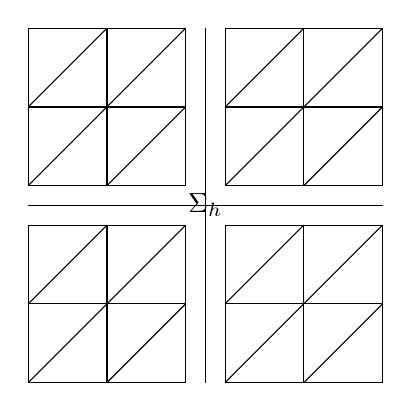
\begin{tikzpicture}  
        \foreach \m in {0,2.5}
        {\foreach \n in {0,2.5}
        {\draw (0+\n,0+\m) -- (2+\n,0+\m);  
        \draw (0+\n,1+\m) -- (2+\n,1+\m);  
        \draw (0+\n,2+\m) -- (2+\n,2+\m);  
        \draw (0+\n,0+\m) -- (0+\n,2+\m); 
        \draw (1+\n,0+\m) -- (1+\n,2+\m);  
        \draw (2+\n,0+\m) -- (2+\n,2+\m);  

        \foreach \y in {0,1}  
        {  
            \draw (\y+\n,0+\m) -- (2+\n,2-\y+\m);
        }  
        \foreach \y in {1,2}  
        {  
            \draw (0+\n,\y+\m) -- (2-\y+\n,2+\m);   
        } } }

        \draw (0, 2.25)--(4.5,2.25);
        \draw (2.25, 4.5)--(2.25,0);
        \node at (2.25,2.25) {$\Sigma_h$}; 
    \end{tikzpicture} 
\end{center}

Also define $$S_h^p(\Sigma_h)=\{v_h\in L_2(\Sigma):v_h|_{\Gamma_{kl}}\in P_p(\Gamma_{kl}),\forall \Gamma_{kl}\in \Sigma_h\}$$

Then take 1D heat equation as above, we need to find $u_h \in S_h^p(\mathscr{T}_N)$ s.t.$\forall v_h\in S_h^p(\mathscr{T}_N)$, $$A(u_h,v_h)=<f,v_h>_Q+<u_0,v_h>_{\Sigma_0}+<g_N,v_h>_{\Sigma_N}$$ 

First we apply this to $Q_i$ respectively. We have local bilinear form: seek $u_h^i,v_h^i \in S_h^p(\mathscr{T}_{N_i})$ s.t. for  $i=1, \ldots, P$
$$A^{(i)}(u_h^i, v_h^i):=a^{(i)}(u_h^i,v_h^i)+b^{(i)}(u_h^i,v_h^i)$$
where 
$$\left\{\begin{aligned}
    a^{(i)}(u_h^i,v_h^i)&=\sum_{l=1}^{N_i}\int_{\tau_h^i}\nabla_x u_h^i\cdot \nabla_x v_h^i d\tau\\
    &-\sum_{\Gamma_{k l} \in \mathcal{I}_{N_{i}}} \int_{\Gamma_{k l}}\left(\left\langle\nabla_{\boldsymbol{x}} u_{h}^{i}\right\rangle_{\Gamma_{k l}} \cdot\left[v_{h}^{i}\right]_{\Gamma_{k l}, \boldsymbol{x}} + \left[u_{h}^{i}\right]_{\Gamma_{k l}, \boldsymbol{x}} \cdot\left\langle\nabla_{\boldsymbol{x}} v_{h}^{i}\right\rangle_{\Gamma_{k l}}\right) \mathrm{d} s \\
    &+\sum_{\Gamma_{k l} \in \mathcal{I}_{N_{i}}} \frac{\sigma}{\overline{h_{k l}}} \int_{\Gamma_{k l}}\left[u_{h}^{i}\right]_{\Gamma_{k l}, \boldsymbol{x}} \cdot\left[v_{h}^{i}\right]_{\Gamma_{k l}, \boldsymbol{x}} \mathrm{d} s\\
    b^{(i)}\left(u_{h}^{i}, v_{h}^{i}\right)&= -\sum_{l=1}^{N_{i}} \int_{\tau_{l}^{i}} u_{h}^{i} \partial_{t} v_{h}^{i} \mathrm{d}+\int_{\Sigma_{T} \cap \partial Q_{i}} u_{h}^{i} v_{h}^{i} \mathrm{d} s 
     +\sum_{\Gamma_{k l} \in \mathcal{I}_{N_{i}} }\int_{\Gamma_{k l}}\left\{u_{h}^{i}\right\}_{\Gamma_{k l}}^{\mathrm{up}}\left[v_{h}^{i}\right]_{\Gamma_{k l}, t} \mathrm{d} s\\
    F^{(i)}\left(v_{h}^{i}\right)&=\left\langle f, v_{h}^{i}\right\rangle_{Q_{i}}+\left\langle u_{0}, v_{h}^{i}\right\rangle_{\Sigma_{0} \cap \partial Q_{i}}+\left\langle g_{N}, v_{h}^{i}\right\rangle_{\Sigma_{N} \cap \partial Q_{i}},
\end{aligned}\right.$$


By using the fact that  $u_{h}^{i}=u_{h}|_{Q_{i}}$  we can split the bilinear form  $A(\cdot, \cdot)$  in a sum over all local bilinear forms  $A^{(i)}(\cdot, \cdot)$  and into four different coupling parts on the interface  $\Sigma_{h}$ 

$$\begin{aligned}
    A\left(u_{h}, v_{h}\right)= & \sum_{i=1}^{P} A^{(i)}\left(u_{h}, v_{h}\right)
    -\sum_{\Gamma_{k l} \in \Sigma_{h}} \int_{\Gamma_{k l}}\left(\left\langle\nabla_{\boldsymbol{x}} u_{h}\right\rangle_{\Gamma_{k l}} \cdot\left[v_{h}\right]_{\Gamma_{k l}, \boldsymbol{x}} +\left[u_{h}\right]_{\Gamma_{k l}, \boldsymbol{x}} \cdot\left\langle\nabla_{\boldsymbol{x}} v_{h}\right\rangle_{\Gamma_{k l}}\right)\mathrm{d} s \\
    & +\sum_{\Gamma_{k l} \in \Sigma_{h}} \frac{\sigma}{\bar{h}_{k l}} \int_{\Gamma_{k l}}\left[u_{h}\right]_{\Gamma_{k l}, \boldsymbol{x}} \cdot\left[v_{h}\right]_{\Gamma_{k l}, \boldsymbol{x}} \mathrm{d} s +\sum_{\Gamma_{k l} \in \Sigma_{h}} \int\left\{u_{h}\right\}_{\Gamma_{k l}}^{\mathrm{up}}\left[v_{h}\right]_{\Gamma_{k l}, t} \mathrm{d} s .
\end{aligned}$$

To reduce the coupling on the interface $\Sigma$, rewrite these terms. Define a new variable $\lambda_h\in S_h^p(\Sigma_h)$ on interface $\Sigma$: $\lambda_h|_{\tau_{kl}}=\frac{1}{2}(u_h|_{\tau_k}+u_h|_{\tau_l})$
\begin{definition}[Hybrid Jump]
    $$[u/\lambda]_{\partial \tau_k}=(u|_{\tau_k}-\lambda)\textbf{n}_k$$
\end{definition}

Then we have $[u]_{\Gamma_{kl}}=2[u/\lambda]_{\partial \tau_k}=2[u/\lambda]_{\partial \tau_l}$, \\
and $[u_h]_{\Gamma_{kl},x}\cdot <\nabla_x v_h>=[u_h/\lambda_h]_{\partial \tau_k,x}\cdot\nabla v_h|_{\tau_k}+[u_h/\lambda_h]_{\partial \tau_l,x}\cdot\nabla v_h|_{\tau_l}$

Hence 
$$\begin{aligned}
    &\sum_{\Gamma_{k l} \in \Sigma_{h}} \int_{\Gamma_{k l}}\left[u_{h}\right]_{\Gamma_{k l}, \boldsymbol{x}} \cdot\left\langle\nabla_{\boldsymbol{x}} v_{h}\right\rangle_{\Gamma_{k l}} \mathrm{d} s\\
    =&\sum_{\Gamma_{k l} \in \Sigma_{h} \Gamma_{k l}}\left[\left[u_{h} / \lambda_{h}\right]_{\partial \tau_{k}, \boldsymbol{x}} \cdot \nabla_{\boldsymbol{x}} v_{h }|_{\tau_{k}}+\left[u_{h} / \lambda_{h}\right]_{\partial \tau_{l}, \boldsymbol{x}} \cdot \nabla_{\boldsymbol{x}} v_{h }|_{\tau_{l}}\right] \mathrm{d} s \\
    =&\sum_{i=1}^{P} \sum_{l=1}^{N_{i}} \sum_{\substack{\Gamma_{k l} \in \Sigma_{h} \\\Gamma_{k l} \subset \partial \tau_{l}^{i} \Gamma_{k l}}}\left[u_{h} / \lambda_{h}\right]_{\partial \tau_{l}^{i}, \boldsymbol{x}} \cdot \nabla_{\boldsymbol{x}} v_{h }|_{\tau_{l}^{i}} \mathrm{d} s .
\end{aligned}$$

Similarly we define $\mu_h=\frac{1}{2}(v_h|_{\tau_k}+v_h|_{\tau_l})\in S_h^p(\Sigma_h)$ for test function $v_h$, and symmetric term turns to
$$\sum_{\Gamma_{k l} \in \Sigma_{h}} \int_{\Gamma_{k l}}\left\langle\nabla_{\boldsymbol{x}} u_{h}\right\rangle_{\Gamma_{k l}} \cdot\left[v_{h}\right]_{\Gamma_{k l}, \boldsymbol{x}} \mathrm{d} s= \\
    \sum_{i=1}^{P} \sum_{l=1}^{N_{i}} \sum_{\substack{\Gamma_{k l} \in \Sigma_{h} \\
    \Gamma_{k l} \subset \partial \tau_{l}^{i}}} \int_{\Gamma_{k l}} \nabla_{\boldsymbol{x}} u_{h }|_{\tau_{l}^{i}}\cdot\left[v_{h} / \mu_{h}\right]_{\partial \tau_{l}^{i}, \boldsymbol{x}} \mathrm{d} s . \\$$
By using conclusion above, we have 
$${\left[u_{h}\right]_{\Gamma_{k l}, \boldsymbol{x}} \cdot\left[v_{h}\right]_{\Gamma_{k l}, \boldsymbol{x}}}    
    =2\left[u_{h} / \lambda_{h}\right]_{\partial \tau_{k}, \boldsymbol{x}} \cdot\left[v_{h} / \mu_{h}\right]_{\partial \tau_{k}, \boldsymbol{x}}
    +2\left[u_{h} / \lambda_{h}\right]_{\partial \tau_{l}, \boldsymbol{x}} \cdot\left[v_{h} / \mu_{h}\right]_{\partial \tau_{l}, \boldsymbol{x}}$$    
    
    With this new representation above the third coupling term of (3.2) can be expressed in the following way
    
$$\begin{aligned}
&\sum_{\Gamma_{k l} \in \Sigma_{h}} \frac{\sigma}{\bar{h}}_{k l} \int_{\Gamma_{k l}}\left[u_{h}\right]_{\Gamma_{k l}, \boldsymbol{x}} \cdot\left[v_{h}\right]_{\Gamma_{k l}, \boldsymbol{x}} \mathrm{d} s \\
=&\sum_{\Gamma_{k l} \in \Sigma_{h}} \frac{2 \sigma}{\bar{h}_{k l}} \int_{\Gamma_{k l}}\left( {\left[u_{h} / \lambda_{h}\right]_{\partial \tau_{k}, \boldsymbol{x}} \cdot\left[v_{h} / \mu_{h}\right]_{\partial \tau_{k}, \boldsymbol{x}} }+\left[u_{h} / \lambda_{h}\right]_{\partial \tau_{l}, \boldsymbol{x}} \cdot\left[v_{h} / \mu_{h}\right]_{\partial \tau_{l}, \boldsymbol{x}}\right) \mathrm{d} s \\
=&\sum_{i=1}^{P} \sum_{l=1}^{N_{i}} \sum_{\substack{\Gamma_{k l} \in \Sigma_{h} \\
\Gamma_{k l} \subset \partial \tau_{l}^{i}}} \frac{2 \sigma}{\overline{h}} \int_{\Gamma_{k l}}\left[u_{h} / \lambda_{h}\right]_{\partial \tau_{l}^{i}, \boldsymbol{x}} \cdot\left[v_{h} / \mu_{h}\right]_{\partial \tau_{l}^{i}, \boldsymbol{x}} \mathrm{d} s .
\end{aligned}$$

\begin{definition}[Hybrid Upwind]
    $$\{u / \lambda\}_{\partial \tau_{k}}^{\operatorname{up}}(\boldsymbol{x}, t):=\left\{\begin{array}{ll}
        u_{\mid \tau_{k}}(\boldsymbol{x}, t) & \text { for } n_{k, t} \geq 0, \\
        0 & \text { for } n_{k, t}=0, \\
        \lambda(\boldsymbol{x}, t) & \text { for } n_{k, t}<0
        \end{array} \quad \text { for }(\boldsymbol{x}, t) \in \Gamma_{k l} .\right.$$
\end{definition}

Then for classical continuous solution, $\lambda=<u>_{\Gamma_{kl}}=u|_{\tau_k}=u|_{\tau_l}$, then 
$$\sum_{\Gamma_{k l} \in \Sigma_{h}} \int_{\Gamma_{k l}}\left\{u_{h}\right\}_{\Gamma_{k l}}^{\text {up }}\left[v_{h}\right]_{\Gamma_{k l}, t} \mathrm{d} s=\sum_{i=1}^{P} \sum_{l=1}^{N_{i}} \sum_{\substack{\Gamma_{k l} \in \Sigma_{h} \\
\Gamma_{k l} \subset \partial \tau_{l}^{i}}}\int_{\Gamma_{kl}}\{u_h/\lambda_h\}_{\partial \tau_l^i}^{up}[v_h/\mu_h]_{\partial \tau_l^i,x}ds$$

So we formulate this by 
$$\begin{aligned}
    &C^{(i)}(u_h,\lambda_h;v_h,\mu_h)\\
    =&-\sum_{l=1}^{N_{i}} \sum_{\substack{\Gamma_{k l} \in \Sigma_{h} \\
    \Gamma_{k l} \subset \partial \tau_{l}^{i}}} \int_{\boldsymbol{l}} \nabla_{\boldsymbol{x} l} u_{h \mid \tau_{l}^{i}} \cdot\left[v_{h} / \mu_{h}\right]_{\partial \tau_{l}^{i}, \boldsymbol{x}} \mathrm{d} s \\
    &+\sum_{l=1}^{N_{i}} \sum_{\substack{\Gamma_{k l} \in \Sigma_{h} \\
    \Gamma_{k l} \subset \partial \tau_{l}^{i}}} \frac{2 \sigma}{\bar{h}_{k l}} \int_{\Gamma_{k l}}\left[u_{h} / \lambda_{h}\right]_{\partial \tau_{l}^{i}, \boldsymbol{x}} \cdot\left[v_{h} / \mu_{h}\right]_{\partial \tau_{l}^{i}, \boldsymbol{x}} \mathrm{d} s \\
    &+\sum_{\substack{l=1}}^{N_{i}} \sum_{\substack{\Gamma_{k l} \in \Sigma_{h} \\
    \Gamma_{k l} \subset \partial \tau_{l}^{i}}} \int_{k l}\left\{u_{h} / \lambda_{h}\right\}_{\partial \tau_{l}^{i}}^{\mathrm{up}}\left[v_{h} / \mu_{h}\right]_{\partial \tau_{l}^{i}, \boldsymbol{x}} \mathrm{d} s . \\
\end{aligned}$$

Finally: seek $u_h\in S_h^p(\mathscr{T}_h)\& \lambda_h\in S_h^p(\Sigma_h)$ s.t. for $\forall v_h\in S_h^p(\mathscr{T}_h)\& \mu_h\in S_h^p(\Sigma_h)$,
$$\sum_{i=1}^{p}\left[A^{(i)}(u_h,v_h)+c^{(i)}(u_h,\lambda_h;v_h,\mu_h)\right]=\sum_{i=1}^{p}F^{(i)}(v_h)$$

For each space-time decomposition
\begin{itemize}
    \item $\mathscr{T}_{N_i}=span\{\phi_l^i\}^{M_i}_l$, for $u_h^i\in S_h^p(\mathscr{T}_{N_i})$, set $u_h^i=\sum_{l=1}^{M_i}U_l^i\phi_l^i(x,t)$
    \item $S_h^p(\Sigma_h)=span\{\psi_n\}_{n=1}^{M_\Sigma}$, for $\lambda_h\in S_h^p(\Sigma_h)$, set $\lambda_h=\sum_{n=1}^{M_\Sigma}\lambda_\Sigma^n\psi_n(x,t)$
\end{itemize}

Then we have the linear form:

$$\left\{\begin{aligned}
    &A_{I I}^{(i)}[k, \ell]  =A^{(i)}\left(\varphi_{\ell}^{i}, \varphi_{k}^{i}\right)+c^{(i)}\left(\varphi_{\ell}^{i}, 0 ; \varphi_{k}^{i}, 0\right) & \text { for } k, \ell=1, \ldots, M_{i}, \\
    &A_{I \Sigma}^{(i)}[k, n]:=c^{(i)}\left(0, \psi_{n} ; \varphi_{k}^{i}, 0\right) & \text { for } k=1, \ldots, M_{i} \text { and } n=1, \ldots, M_{\Sigma} \\
    &A_{\Sigma I}^{(i)}[m, \ell]  :=c^{(i)}\left(\varphi_{\ell}^{i}, 0 ; 0, \psi_{m}\right) & \text { for } m=1, \ldots, M_{\Sigma} \text { and } \ell=1, \ldots, M_{i}\\
    &A_{\Sigma \Sigma}[m, n]:=\sum_{i=1}^{P} c^{(i)}\left(0, \psi_{n} ; 0, \psi_{m}\right) & \text { for } m, n=1, \ldots, M_{\Sigma} .
\end{aligned}\right.$$
    
and RHS
$$F_{I}^{(i)}[k]:=F^{(i)}\left(\varphi_{k}^{i}\right) \quad \text { for } k=1, \ldots, M_{i} .$$

\paragraph*{Matrix form}
$$\left(\begin{array}{ccccc}
    A_{I I}^{(1)} & & & & A_{I \Sigma}^{(1)} \\
    & A_{I I}^{(2)} & & & A_{I \Sigma}^{(2)} \\
    & & \ddots & & \vdots \\
    & & & A_{I I}^{(P)} & A_{I \Sigma}^{(P)} \\
    A_{\Sigma I}^{(1)} & A_{\Sigma I}^{(2)} & \cdots & A_{\Sigma I}^{(P)} & A_{\Sigma \Sigma}
    \end{array}\right)\left(\begin{array}{c}
    \boldsymbol{u}_{I}^{(1)} \\
    \boldsymbol{u}_{I}^{(2)} \\
    \vdots \\
    \boldsymbol{u}_{I}^{(P)} \\
    \boldsymbol{\lambda}_{\Sigma}
    \end{array}\right)=\left(\begin{array}{c}
    \boldsymbol{f}_{I}^{(1)} \\
    \boldsymbol{f}_{I}^{(2)} \\
    \vdots \\
    \boldsymbol{f}_{I}^{(P)} \\
    \mathbf{0}
\end{array}\right) .$$
    

\section{About Parallel Computation}
Parallelization $\Rightarrow$ Multigrid Method.


